\documentclass{standalone}
\usepackage{tikz}
\usetikzlibrary{patterns, positioning}


\begin{document}
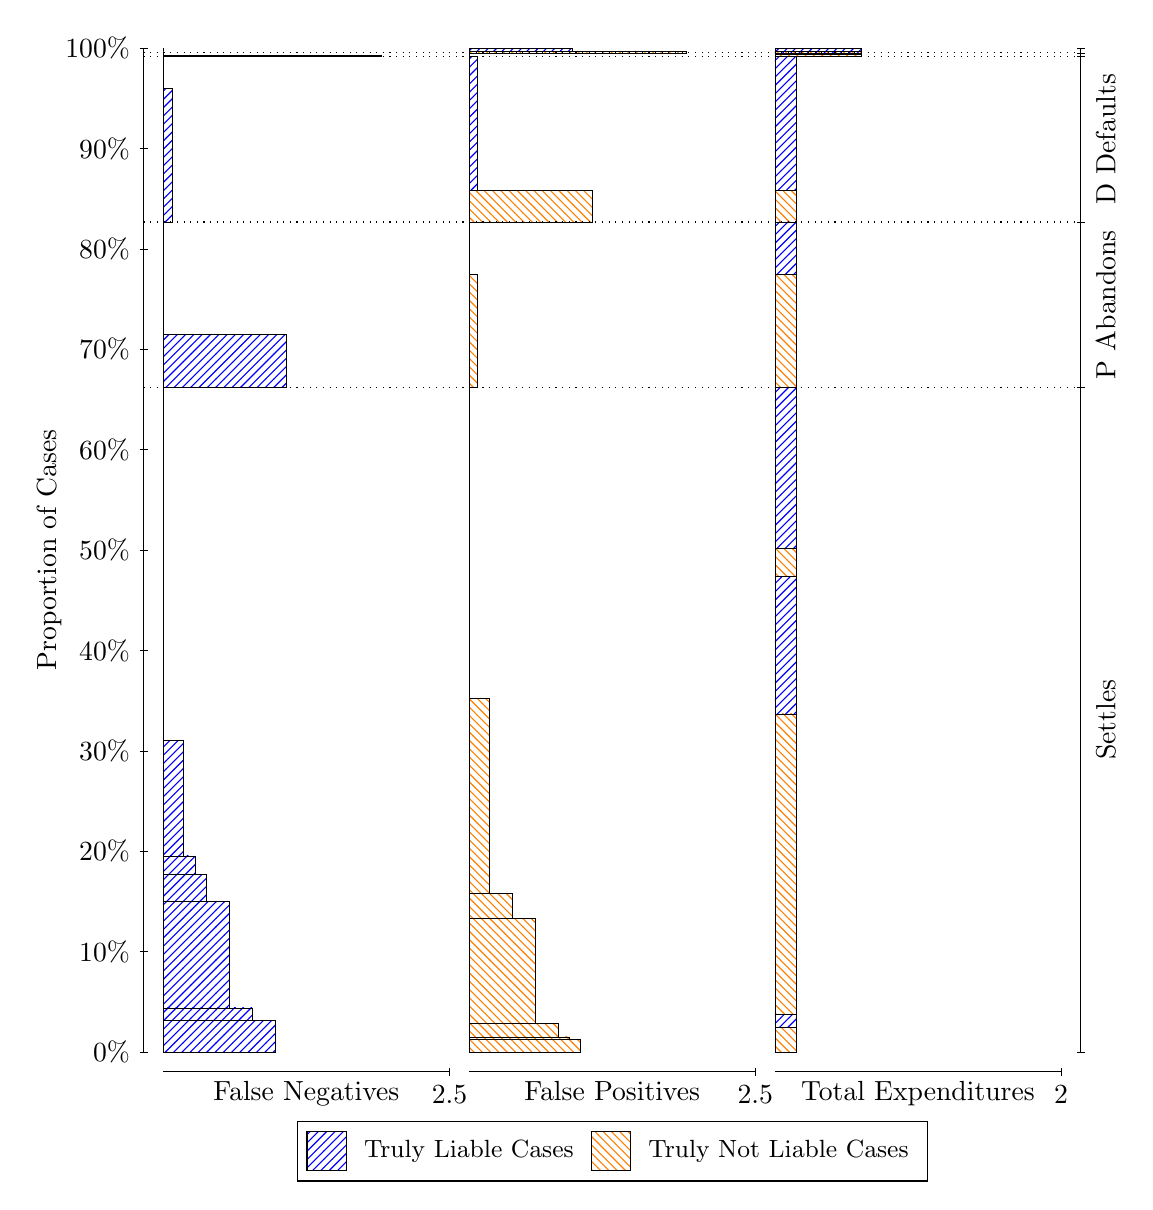
\begin{tikzpicture}
\draw[black, very thin] (1.5,1.75) -- (1.5,14.5);
\node[rotate=90, text=black, anchor=center] at (0.3, 8.125) {Proportion of Cases};
\draw[black, very thin] (1.45,1.75) -- (1.55,1.75);
\node[text=black, anchor=east] at (1.45, 1.75) {0\%};
\draw[black, very thin] (1.45,3.025) -- (1.55,3.025);
\node[text=black, anchor=east] at (1.45, 3.025) {10\%};
\draw[black, very thin] (1.45,4.3) -- (1.55,4.3);
\node[text=black, anchor=east] at (1.45, 4.3) {20\%};
\draw[black, very thin] (1.45,5.575) -- (1.55,5.575);
\node[text=black, anchor=east] at (1.45, 5.575) {30\%};
\draw[black, very thin] (1.45,6.85) -- (1.55,6.85);
\node[text=black, anchor=east] at (1.45, 6.85) {40\%};
\draw[black, very thin] (1.45,8.125) -- (1.55,8.125);
\node[text=black, anchor=east] at (1.45, 8.125) {50\%};
\draw[black, very thin] (1.45,9.4) -- (1.55,9.4);
\node[text=black, anchor=east] at (1.45, 9.4) {60\%};
\draw[black, very thin] (1.45,10.675) -- (1.55,10.675);
\node[text=black, anchor=east] at (1.45, 10.675) {70\%};
\draw[black, very thin] (1.45,11.95) -- (1.55,11.95);
\node[text=black, anchor=east] at (1.45, 11.95) {80\%};
\draw[black, very thin] (1.45,13.225) -- (1.55,13.225);
\node[text=black, anchor=east] at (1.45, 13.225) {90\%};
\draw[black, very thin] (1.45,14.5) -- (1.55,14.5);
\node[text=black, anchor=east] at (1.45, 14.5) {100\%};

\draw[black, very thin] (13.4,1.75) -- (13.4,14.5);
\draw[black, very thin] (13.35,1.75) -- (13.45,1.75);
\node[anchor=west] at (13.35, 1.75) {};
\draw[black, very thin] (13.35,10.192) -- (13.45,10.192);
\node[anchor=west] at (13.35, 10.192) {};
\draw[black, very thin] (13.35,12.291) -- (13.45,12.291);
\node[anchor=west] at (13.35, 12.291) {};
\draw[black, very thin] (13.35,14.389) -- (13.45,14.389);
\node[anchor=west] at (13.35, 14.389) {};
\draw[black, very thin] (13.35,14.439) -- (13.45,14.439);
\node[anchor=west] at (13.35, 14.439) {};
\draw[black, very thin] (13.35,14.5) -- (13.45,14.5);
\node[anchor=west] at (13.35, 14.5) {};

\draw[black, very thin, pattern color=blue, pattern=north east lines] (1.75,1.75) rectangle (3.167,2.1468);
\draw[black, very thin, pattern color=blue, pattern=north east lines] (1.75,2.1468) rectangle (2.8763,2.3087);
\draw[black, very thin, pattern color=blue, pattern=north east lines] (1.75,2.3087) rectangle (2.731,2.3112);
\draw[black, very thin, pattern color=blue, pattern=north east lines] (1.75,2.3112) rectangle (2.5857,3.6597);
\draw[black, very thin, pattern color=blue, pattern=north east lines] (1.75,3.6597) rectangle (2.295,4.0011);
\draw[black, very thin, pattern color=blue, pattern=north east lines] (1.75,4.0011) rectangle (2.1497,4.2412);
\draw[black, very thin, pattern color=blue, pattern=north east lines] (1.75,4.2412) rectangle (2.0043,5.7023);
\draw[black, very thin, pattern color=orange, pattern=north west lines] (1.75,5.7023) rectangle (1.75,10.192);
\draw[black, very thin, pattern color=blue, pattern=north east lines] (1.75,10.192) rectangle (3.3123,10.859);
\draw[black, very thin, pattern color=orange, pattern=north west lines] (1.75,10.859) rectangle (1.75,12.291);
\draw[black, very thin, pattern color=blue, pattern=north east lines] (1.75,12.291) rectangle (1.859,13.985);
\draw[black, very thin, pattern color=orange, pattern=north west lines] (1.75,13.985) rectangle (1.75,14.389);
\draw[black, very thin, pattern color=blue, pattern=north east lines] (1.75,14.389) rectangle (4.5113,14.408);
\draw[black, very thin, pattern color=orange, pattern=north west lines] (1.75,14.408) rectangle (1.75,14.439);
\draw[black, very thin, pattern color=orange, pattern=north west lines] (1.75,14.439) rectangle (1.75,14.457);
\draw[black, very thin, pattern color=blue, pattern=north east lines] (1.75,14.457) rectangle (1.75,14.5);
\draw[black, very thin, pattern color=orange, pattern=north west lines] (5.6333,1.75) rectangle (7.0503,1.908);
\draw[black, very thin, pattern color=orange, pattern=north west lines] (5.6333,1.908) rectangle (6.905,1.943);
\draw[black, very thin, pattern color=orange, pattern=north west lines] (5.6333,1.943) rectangle (6.7597,2.1089);
\draw[black, very thin, pattern color=orange, pattern=north west lines] (5.6333,2.1089) rectangle (6.469,3.4469);
\draw[black, very thin, pattern color=orange, pattern=north west lines] (5.6333,3.4469) rectangle (6.3237,3.4481);
\draw[black, very thin, pattern color=orange, pattern=north west lines] (5.6333,3.4481) rectangle (6.1783,3.7622);
\draw[black, very thin, pattern color=orange, pattern=north west lines] (5.6333,3.7622) rectangle (5.8877,6.2395);
\draw[black, very thin, pattern color=blue, pattern=north east lines] (5.6333,6.2395) rectangle (5.6333,10.192);
\draw[black, very thin, pattern color=orange, pattern=north west lines] (5.6333,10.192) rectangle (5.7423,11.624);
\draw[black, very thin, pattern color=blue, pattern=north east lines] (5.6333,11.624) rectangle (5.6333,12.291);
\draw[black, very thin, pattern color=orange, pattern=north west lines] (5.6333,12.291) rectangle (7.1957,12.695);
\draw[black, very thin, pattern color=blue, pattern=north east lines] (5.6333,12.695) rectangle (5.7423,14.389);
\draw[black, very thin, pattern color=orange, pattern=north west lines] (5.6333,14.389) rectangle (5.6333,14.421);
\draw[black, very thin, pattern color=blue, pattern=north east lines] (5.6333,14.421) rectangle (5.6333,14.439);
\draw[black, very thin, pattern color=orange, pattern=north west lines] (5.6333,14.439) rectangle (8.3947,14.457);
\draw[black, very thin, pattern color=blue, pattern=north east lines] (5.6333,14.457) rectangle (6.9413,14.5);
\draw[black, very thin, pattern color=orange, pattern=north west lines] (9.5167,1.75) rectangle (9.7892,2.0653);
\draw[black, very thin, pattern color=blue, pattern=north east lines] (9.5167,2.0653) rectangle (9.7892,2.2297);
\draw[black, very thin, pattern color=orange, pattern=north west lines] (9.5167,2.2297) rectangle (9.7892,6.045);
\draw[black, very thin, pattern color=blue, pattern=north east lines] (9.5167,6.045) rectangle (9.7892,7.7903);
\draw[black, very thin, pattern color=orange, pattern=north west lines] (9.5167,7.7903) rectangle (9.7892,8.1492);
\draw[black, very thin, pattern color=blue, pattern=north east lines] (9.5167,8.1492) rectangle (9.7892,10.192);
\draw[black, very thin, pattern color=orange, pattern=north west lines] (9.5167,10.192) rectangle (9.7892,11.624);
\draw[black, very thin, pattern color=blue, pattern=north east lines] (9.5167,11.624) rectangle (9.7892,12.291);
\draw[black, very thin, pattern color=orange, pattern=north west lines] (9.5167,12.291) rectangle (9.7892,12.695);
\draw[black, very thin, pattern color=blue, pattern=north east lines] (9.5167,12.695) rectangle (9.7892,14.389);
\draw[black, very thin, pattern color=orange, pattern=north west lines] (9.5167,14.389) rectangle (10.607,14.421);
\draw[black, very thin, pattern color=blue, pattern=north east lines] (9.5167,14.421) rectangle (10.607,14.439);
\draw[black, very thin, pattern color=orange, pattern=north west lines] (9.5167,14.439) rectangle (10.607,14.457);
\draw[black, very thin, pattern color=blue, pattern=north east lines] (9.5167,14.457) rectangle (10.607,14.5);
\draw[black, dotted] (1.5,10.192) -- (13.4,10.192);
\draw[black, dotted] (1.5,12.291) -- (13.4,12.291);
\draw[black, dotted] (1.5,14.389) -- (13.4,14.389);
\draw[black, dotted] (1.5,14.439) -- (13.4,14.439);
\draw[black, very thin] (1.75,1.5) -- (5.3833,1.5);
\node[text=black, anchor=north] at (3.5667, 1.5) {False Negatives};
\draw[black, very thin] (5.3833,1.45) -- (5.3833,1.55);
\node[text=black, anchor=north] at (5.3833, 1.45) {2.5};

\draw[black, very thin] (5.6333,1.5) -- (9.2667,1.5);
\node[text=black, anchor=north] at (7.45, 1.5) {False Positives};
\draw[black, very thin] (9.2667,1.45) -- (9.2667,1.55);
\node[text=black, anchor=north] at (9.2667, 1.45) {2.5};

\draw[black, very thin] (9.5167,1.5) -- (13.15,1.5);
\node[text=black, anchor=north] at (11.333, 1.5) {Total Expenditures};
\draw[black, very thin] (13.15,1.45) -- (13.15,1.55);
\node[text=black, anchor=north] at (13.15, 1.45) {2};

\node[text=black, centered, rotate=90] at (13.72, 5.9709) {Settles};
\node[text=black, centered, rotate=90] at (13.72, 11.241) {P Abandons};
\node[text=black, centered, rotate=90] at (13.72, 13.34) {D Defaults};



\draw (7.449999999999999,1.5) node[draw=none] (baseCoordinate) {};
\begin{scope}[align=center]
        \matrix[scale=0.5, draw=black, below=0.5cm of baseCoordinate, nodes={draw}, column sep=0.1cm]{
            \node[rectangle, draw, minimum width=0.5cm, minimum height=0.5cm, pattern color=blue, pattern=north east lines] {}; &
            \node[draw=none, font=\small, text=black] (B) {Truly Liable Cases}; &
            \node[rectangle, draw, minimum width=0.5cm, minimum height=0.5cm, pattern color=orange, pattern=north west lines] {}; &
            \node[draw=none, font=\small, text=black] (B) {Truly Not Liable Cases}; \\
            };
\end{scope}

\end{tikzpicture}
\end{document}